% Page budget: 8 pages
\chapter{חלופות תכן והחלטה}

הפרק בוחר בין שלוש גישות תכן שונות עקרונית באמצעות מטריצת החלטה משוקללת, ומראה שהחלופה ההיברידית מובילה בכל תרחישי בדיקת הרגישות. לאחר מכן הוא מציג את הארכיטקטורה ואת זרימת הנתונים של המערכת הנבחרת, ומסיים בהגדרה מנומקת של החדשנות. המשקלים והציונים בפרק הם הערכה של הצוות שאושרה על ידי חבריו, ואינם עובדות ממקור חיצוני. לכן הם מוצגים כהערכה בכל מקום שבו הם מופיעים, והדוח אינו מייחס להם תוקף של מדידה.

\section{חלופות תכן}
\label{sec:ch5-alternatives}
שלוש החלופות נבדלות בשאלה היסודית היכן נמצאת יכולת היצירה של הווידאו: בתוך הצוות, אצל ספק חיצוני, או בשילוב ביניהם. טבלה~\ref{tab:ch5-alternatives} מציגה לכל חלופה את היתרון העיקרי ואת המחיר שלו, והיא מראה שאין חלופה שאינה דורשת פשרה.

\begin{table}[h]
  \centering
  \caption{שלוש חלופות התכן: יתרון ומחיר}
  \label{tab:ch5-alternatives}
  \small
  \begin{tabular}{p{3.6cm} p{4.6cm} p{4.6cm}}
    \headrow \hcell{חלופה} & \hcell{יתרון} & \hcell{מחיר} \\
    \textbf{א׳:} מודל וידאו ייעודי שאומן או כוונן בידי הצוות & שליטה מלאה ועלות שולית נמוכה בהמשך & עלות פיתוח וחישוב גבוהה מאוד וזמן פיתוח ארוך \\ \rowrule
    \textbf{ב׳:} שכבת סוכנים מעל מודלים מסחריים דרך \textenglish{API} & זמן פיתוח קצר ואיכות גבוהה & תלות בספקים ועלות לדקה \\ \rowrule
    \textbf{ג׳:} היברידי: מודלים בקוד פתוח מקומית, ו־\textenglish{API} רק לשוטים קשים & איזון בין עלות לשליטה & מורכבות תפעולית, ונדרשת יחידת עיבוד גרפי (\textenglish{GPU}) \\
  \end{tabular}
\end{table}

חלופה א׳ מעניקה שליטה מלאה, אך היא דורשת אימון והערכה של מודל וידאו, ומשימה כזו אינה ניתנת להשלמה בסמסטר של ארבעה־עשר שבועות. חלופה ב׳ מקצרת את הפיתוח משום שהמודלים מוכנים, אך כל שנייה שנוצרת מחויבת, והמוצר חשוף לשינויי מחיר, ממשק ומדיניות של הספק. חלופה ג׳ מפצלת את העומס: מודלים בקוד פתוח מייצרים את רוב השוטים במקום, וקריאה לשירות חיצוני נשמרת לשוטים הקשים בלבד. המחיר הוא מורכבות תפעולית, כי נדרשים הקמת תשתית \textenglish{GPU} ולוגיקת ניתוב בין המודלים.

ההבדל בין שלוש החלופות הוא עקרוני ולא כמותי. בחלופה א׳ הצוות הוא בעל המודל, ולכן כל שיפור באיכות הוא עבודת מחקר שלו. בחלופה ב׳ המודל שייך לספק, והצוות מתמקד בתזמור ובזיכרון העלילה. בחלופה ג׳ הצוות בוחר לכל שוט את המקור המתאים ביותר, ולכן הוא מחזיק גם מודלים וגם חוזים עם ספקים. שלוש הגישות מובילות לפרופילים שונים של סיכון: חלופה א׳ מסתכנת בכך שהפרויקט לא יושלם, חלופה ב׳ בכך שמחיר או מדיניות של ספק יפגעו במוצר, וחלופה ג׳ בכך שהמורכבות התפעולית תחרוג מהיכולת של צוות קטן. הפרויקט עוסק בניהול רציפות עלילתית ולא באימון מודלי וידאו, ולכן חלופה א׳ מרחיקה את הצוות מהשאלה המרכזית שלו, בעוד שחלופות ב׳ ו־ג׳ מותירות את המאמץ בשכבת הסוכנים והזיכרון.

מבחינה טכנית, חלופה א׳ מחייבת איסוף נתוני וידאו, כוונון של מודל קיים וכתיבת תשתית הערכה, ובנוסף בניית קול וסנכרון שפתיים בעברית מאפס. הסיכון המרכזי הוא שהמאמץ ייבלע בהנדסת מודל בלי שיגיע לניהול הסדרה, ולכן הציון הנמוך בזמן הפיתוח ובאיכות, והציון הגבוה בתלות בספק ובפרטיות, נובעים כולם מאותה בחירה: הכול נשאר בבית.

חלופה ב׳ בנויה משכבת תזמור דקה מעל שירותי תמונה, וידאו וקול של ספקים. הסיכון המרכזי הוא חשיפה: שינוי מחיר, ממשק או מדיניות תוכן אצל ספק פוגע ישירות במוצר, ותמיכת העברית משתנה בין ספק לספק ואינה אחידה בין תמונה, קול וסנכרון שפתיים. לכן קיבלה חלופה זו את הציון הגבוה ביותר באיכות ובזמן הפיתוח, ואת הנמוך ביותר בתלות בספק.

חלופה ג׳ מוסיפה לשכבת התזמור רכיב ניתוב, מודלים פתוחים מקומיים וספק חיצוני כגיבוי. הסיכון המרכזי הוא עומס תפעולי על צוות קטן, ולכן זמן הפיתוח קיבל \textenglish{3} בלבד. האיכות גם היא נמוכה מזו של \textenglish{API} טהור, משום שרוב השוטים נוצרים במודלים פתוחים, אך העלות, העברית והפרטיות משתפרות, כי מודלי דיבור פתוחים בעברית נבחרים מקומית ורוב המידע אינו עוזב את המערכת.

\section{מטריצת החלטה}
\subsection{קריטריונים ומשקלים}
שישה קריטריונים נבחרו להשוואה, והמשקלים שלהם נקבעו לפני מתן הציונים, כדי שהציונים לא ישפיעו על חשיבות הקריטריונים. סכום המשקלים הוא \textenglish{1.0}. עקביות ואיכות קיבלה את המשקל הגבוה ביותר (\textenglish{0.25}) משום שהיא לב הבעיה שהפרויקט בא לפתור. עלות לדקה ותמיכה בעברית קיבלו \textenglish{0.20} כל אחד, כי הראשונה מגבילה את כדאיות ההפקה והשנייה היא מאפיין מגדיר של קהל היעד. זמן הפיתוח קיבל \textenglish{0.15} בשל מגבלת הסמסטר. תלות בספק ופרטיות ושליטה בקניין רוחני קיבלו \textenglish{0.10} כל אחד. המשקלים הם הערכה של הצוות ואושרו על ידו.

הסדר בין הקריטריונים משקף את מבנה הפרויקט. שני הקריטריונים הראשונים, עקביות ואיכות ועלות, יחד מהווים \textenglish{0.45} מהמשקל, משום שהם קובעים אם הסדרה ראויה לצפייה ואם אפשר להפיק אותה שוב ושוב. עברית נמדדת בנפרד ולא נכללת באיכות, כי חלופה יכולה להיות איכותית חזותית ועדיין לא לתמוך בקול ובכתוביות בעברית. שני הקריטריונים האחרונים קיבלו משקל נמוך יותר משום שהם משפיעים בעיקר על סיכון עתידי ולא על ההפקה בסמסטר הקרוב. כפי שמראה ניתוח הרגישות שלהלן, ההכרעה אינה תלויה בדיוק של משקלים אלה.

\subsection{ציונים וחישוב}
כל חלופה קיבלה ציון בין \textenglish{1} ל־\textenglish{5} בכל קריטריון, כשציון גבוה הוא תמיד טוב יותר: בעלות הציון \textenglish{5} פירושו הזול ביותר לדקה, ובתלות בספק \textenglish{5} פירושו התלות הנמוכה ביותר. הציון המשוקלל של חלופה $j$ מחושב לפי משוואה~\eqref{eq:ch5-score}:
\begin{equation}
  S_j = \sum_{i=1}^{6} w_i \, c_{ij}, \qquad \sum_{i=1}^{6} w_i = 1
  \label{eq:ch5-score}
\end{equation}
כאשר $w_i$ הוא משקל הקריטריון $i$, ו־$c_{ij}$ הוא ציון חלופה $j$ בקריטריון $i$. טבלה~\ref{tab:ch5-matrix} מציגה את המשקלים, את הציונים ואת הסכומים. הציונים הם הערכת צוות שאושרה על ידו ואינם נשענים על מקור, והנימוק לכל ציון מתועד בקובץ הנתונים של הפרויקט.

\begin{table}[h]
  \centering
  \caption{מטריצת החלטה משוקללת (משקלים וציונים: הערכת הצוות)}
  \label{tab:ch5-matrix}
  \small
  \begin{tabular}{p{4.6cm} c c c c}
    \headrow \hcell{קריטריון} & \hcell{משקל $w_i$} & \hcell{א׳} & \hcell{ב׳} & \hcell{ג׳} \\
    עקביות ואיכות & 0.25 & 2 & 4 & 3 \\ \rowrule
    עלות לדקה & 0.20 & 3 & 2 & 4 \\ \rowrule
    תמיכה בעברית & 0.20 & 3 & 3 & 4 \\ \rowrule
    זמן פיתוח & 0.15 & 1 & 5 & 3 \\ \rowrule
    תלות בספק & 0.10 & 5 & 1 & 3 \\ \rowrule
    פרטיות ושליטה בקניין רוחני & 0.10 & 5 & 2 & 4 \\ \rowrule
    \textbf{ציון משוקלל $S_j$} & \textbf{1.00} & \textbf{2.85} & \textbf{3.05} & \textbf{3.50} \\
  \end{tabular}
\end{table}

הנימוקים לציונים מבוססים על שיקול דעת של הצוות. בעקביות ואיכות קיבלה חלופה א׳ את הציון \textenglish{2}, משום שצוות קטן אינו צפוי להשיג בכוונון עצמי את האיכות החזותית של מודלי וידאו מובילים, וחלופה ב׳ קיבלה \textenglish{4} משום שמודלים מסחריים מספקים את האיכות הטובה ביותר הזמינה כיום. בעלות לדקה קיבלה חלופה ב׳ את הציון הנמוך \textenglish{2}, כי כל שנייה שנוצרת מחויבת. בזמן הפיתוח קיבלה חלופה א׳ את הציון \textenglish{1}, משום שאימון והערכה של מודל וידאו אינם משתלבים בסמסטר אחד. בתמיכה בעברית קיבלה חלופה ג׳ \textenglish{4}, כי אפשר לבחור מקומית מודלי דיבור פתוחים בעברית ולהשאיר ספק חיצוני כגיבוי. בתלות בספק ובפרטיות קיבלה חלופה ב׳ את הציונים הנמוכים, כי תסריטים ותמונות דמויות נשלחים לשירותי צד שלישי. מכיוון שהציונים אינם נשענים על מקור, הם נבחנים שוב בסמסטר ב׳ מול מדידות.

חלופה ג׳ מובילה עם \textenglish{3.50}, אחריה חלופה ב׳ עם \textenglish{3.05} וחלופה א׳ עם \textenglish{2.85}. איור~\ref{fig:ch5-decision} מפרק כל ציון לתרומות של הקריטריונים ($w_i c_{ij}$), ומאפשר לראות מהיכן נובע ההפרש. חלופה ב׳ מקבלת תרומה גבוהה מאיכות ומזמן פיתוח, אך תרומתה קטנה בעלות, בתלות בספק ובפרטיות. חלופה א׳ מקבלת תרומה גבוהה מתלות בספק ומפרטיות, אך כמעט אינה מקבלת תרומה מזמן פיתוח. חלופה ג׳ אינה הטובה ביותר בקריטריון בודד כלשהו מלבד עלות ועברית, אך היא היחידה שאינה מקבלת ציון נמוך מ־\textenglish{3} באף קריטריון, ולכן סכומה הגבוה ביותר.

\begin{figure}[h]
  \centering
  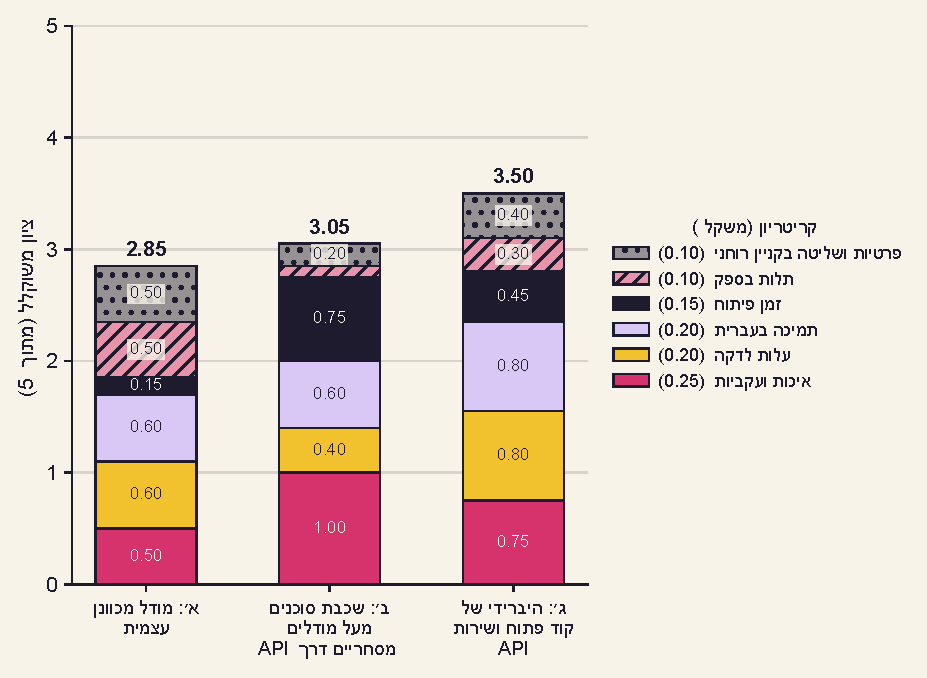
\includegraphics[width=0.8\textwidth]{figures/ch5_decision.pdf}
  \caption{תרומת כל קריטריון לציון המשוקלל של כל חלופה (משקלים וציונים: הערכת הצוות)}
  \label{fig:ch5-decision}
\end{figure}

\subsection{ניתוח רגישות}
בדיקת הרגישות בוחנת האם ההכרעה תלויה במשקלים שנבחרו. כל משקל הוזז בנפרד ב־\textenglish{0.1} כלפי מעלה וכלפי מטה, ושאר המשקלים הוקטנו או הוגדלו באופן יחסי כך שהסכום נשאר \textenglish{1.0}. בסך הכול נבדקו שנים־עשר תרחישים בנוסף למקרה הבסיס, והחישוב בוצע בקוד של הפרויקט. חלופה ג׳ ניצחה בכולם. ציונה נע בין \textenglish{3.43} ל־\textenglish{3.57}, והפער הקטן ביותר שלה מחלופה ב׳ נרשם כשמשקל זמן הפיתוח עלה ל־\textenglish{0.25}: \textenglish{3.44} מול \textenglish{3.28}, כלומר פער של \textenglish{0.16}. חלופה א׳ עקפה את חלופה ב׳ בארבעה תרחישים, אך לא את חלופה ג׳. בשני תרחישים משקל קריטריון אחד הופחת ל־\textenglish{0}, ובהם ג׳ עדיין ניצחה.

הפירוט מלמד על האופי של כל חלופה. חלופה ב׳ רגישה ביותר למשקל זמן הפיתוח: כשמשקלו יורד ל־\textenglish{0.05} ציונה יורד ל־\textenglish{2.82}, וכשהוא עולה ל־\textenglish{0.25} הציון עולה ל־\textenglish{3.28}. היא רגישה גם למשקלי האיכות והעלות: כשמשקל האיכות יורד ל־\textenglish{0.15} או כשמשקל העלות עולה ל־\textenglish{0.30}, ציונה יורד ל־\textenglish{2.92}. חלופה א׳ מרוויחה מהגדלת משקל התלות בספק ומשקל הפרטיות, ובכל אחד מהם היא מגיעה ל־\textenglish{3.09}, אך עדיין נשארת מאחורי חלופה ג׳ שמגיעה ל־\textenglish{3.44} ול־\textenglish{3.56} בהתאמה. חלופה ג׳ יציבה כי היא ממוצעת: אין לה ציון חריג כלפי מעלה או מטה, ולכן שינוי במשקל אחד אינו מזיז אותה בצורה חדה.

חשוב להדגיש את גבול המסקנה. הבדיקה מראה שההכרעה יציבה ביחס לשינוי המשקלים, אך אינה בודקת שינוי של הציונים עצמם, והציונים הם הערכה. שינוי בציון אחד, למשל ירידה באיכות של מודלים בקוד פתוח, עלול לצמצם את הפער, והדבר יידרש בדיקה חוזרת בסמסטר ב׳ לאחר מדידה בפועל.

\begin{directornote}
המטריצה לא נועדה להוכיח שחלופה ג׳ ״נכונה״, אלא לחשוף על אילו הנחות היא נשענת. ההנחה הרגישה ביותר היא הציון ״ג׳ בעקביות ואיכות: 3״. לכן המדידה הראשונה בסמסטר ב׳ תהיה השוואת איכות של שוט מקומי מול שוט דרך \textenglish{API}.
\end{directornote}

\section{הארכיטקטורה הנבחרת}
\subsection{ארכיטקטורת המערכת}
הארכיטקטורה היא צוות של שישה סוכנים הפועלים במעגל סביב זיכרון משותף, והיא מיישמת את חלופה ג׳ בשכבת התזמור. איור~\ref{fig:ch5-architecture} מציג את הסדר: שומר ספר הסדרה מספק את מצב העולם, כותב העלילה מציע את הפרק, והבמאי מתרגם אותו לסטוריבורד ולשוטים. מתזמר הייצור מפעיל את המודלים ומחליט איזה שוט יוצר מקומית ואיזה דרך \textenglish{API}, בדיוק כפי שחלופה ג׳ מגדירה. בודק הרציפות משווה את התוצר לספר הסדרה ומתריע על סתירות, ומנתח הקהל מזין את הצעות הפרק הבא. התוצאה חוזרת לשומר ספר הסדרה, וכך המעגל נסגר.

\begin{figure}[h]
  \centering
  \begin{tikzpicture}[
      box/.style={draw, rounded corners=3pt, minimum width=3.8cm, minimum height=1.7cm, align=center, text width=3.6cm, inner sep=3pt, font=\small},
      keep/.style={box, very thick, fill=black!8},
      arr/.style={->, thick}]
    \node[keep] (a) at (5,1.6) {\textbf{1. שומר ספר הסדרה}\\ זיכרון עולם ועלילה};
    \node[box]  (b) at (0,1.6) {\textbf{2. כותב העלילה}\\ הצעת פרק};
    \node[box]  (c) at (-5,1.6) {\textbf{3. במאי}\\ סטוריבורד ושוטים};
    \node[box]  (d) at (-5,-1.6) {\textbf{4. מתזמר הייצור}\\ ניתוב בין מודלים};
    \node[box]  (e) at (0,-1.6) {\textbf{5. בודק רציפות}\\ זיהוי סתירות};
    \node[box]  (f) at (5,-1.6) {\textbf{6. מנתח קהל}\\ תגובות וצפיות};
    \draw[arr] (a) -- (b);
    \draw[arr] (b) -- (c);
    \draw[arr] (c) -- (d);
    \draw[arr] (d) -- (e);
    \draw[arr] (e) -- (f);
    \draw[arr] (f) -- (a);
  \end{tikzpicture}
  \caption{ארכיטקטורת צוות הסוכנים: מעגל סגור סביב ספר הסדרה}
  \label{fig:ch5-architecture}
\end{figure}

תפקידי הסוכנים מוגדרים לפי הקלט והפלט של כל אחד. שומר ספר הסדרה מקבל פרק מוגמר ומחלץ ממנו אירועים, יחסים ושינויים במצב הדמויות, וכותב אותם לספר. כותב העלילה קורא את הספר ואת בקשת המשתמש ומפיק תסריט לפרק הבא. הבמאי מפרק את התסריט לסצנות, לסטוריבורד ולשוטים, ומציין לכל שוט אילו דמויות מופיעות בו. מתזמר הייצור מקבל רשימת שוטים ומפעיל מודלי תמונה, וידאו וקול. בודק הרציפות מקבל את הפרק ואת הספר, ומחזיר רשימת סתירות אפשריות עם הנימוק לכל אחת. מנתח הקהל מקבל נתוני צפייה ותגובות אחרי הפרסום ומחזיר הצעות להמשך. חלוקה כזו מאפשרת לבדוק כל סוכן בנפרד, ולהחליף את המודל שמאחוריו מבלי לשנות את שאר המעגל, וזו התכונה שמצדיקה את בחירת חלופה ג׳ שבה הספקים ניתנים להחלפה.

הזרימה בין הסוכנים מועברת במבנים מוגדרים ולא בטקסט חופשי. בין שומר ספר הסדרה לכותב העלילה עובר מצב עולם: דמויות, אירועים ויחסים. בין כותב העלילה לבמאי עובר תסריט, ובין הבמאי למתזמר רשימת שוטים שלכל אחד מהם תיאור חזותי ורשימת דמויות. המתזמר מעביר לבודק הרציפות את הפרק שנוצר, והבודק מחזיר לבמאי או למתזמר דרישת תיקון כשנמצאה סתירה. מנתח הקהל מעביר לכותב העלילה הצעות מבוססות תגובות. בנוסף, ההפרדה מאפשרת לתעד כל מעבר, ולכן אפשר לדעת איזה סוכן גרם לשגיאה.

הארכיטקטורה קרובה לצוות ההפקה של \textenglish{StoryAgent} \cite{hu2024storyagent}, וכן לתפקיד הבמאי שמוצע במאמר \textenglish{VideoDirectorGPT} \cite{lin2023videodirectorgpt}. ההבדל הוא בשני הסוכנים שאינם מופיעים בהם כמטרה: שומר ספר הסדרה, שמחזיק מצב עלילה בין פרקים, ובודק הרציפות, שמשווה את הפרק החדש למצב הזה.

\subsection{תרשים זרימת נתונים}
תרשים זרימת הנתונים מראה מה עובר בין הרכיבים מרגע הקלט ועד הפרק המוגמר, ואיפה ספר הסדרה משמש כזיכרון משותף. כפי שמוצג באיור~\ref{fig:ch5-dataflow}, הקלט הוא טקסט או דיבור בעברית, והוא מומר לטקסט ומובן בשלב הראשון. שלבי הכתיבה והבימוי קוראים את ספר הסדרה כדי להישאר נאמנים לעולם, בודק הרציפות קורא אותו כדי לאתר סתירות, וספר הסדרה מתעדכן בסוף עם הפרק שנוצר. השלב של כתוביות ושמע בעברית נעשה לפני הפלט, כדי שהכתוביות יוצגו מימין לשמאל.

\begin{figure}[h]
  \centering
  \begin{tikzpicture}[
      box/.style={draw, rounded corners=3pt, minimum width=3.1cm, minimum height=1.5cm, align=center, text width=2.9cm, inner sep=3pt, font=\small},
      mem/.style={draw, very thick, rounded corners=3pt, fill=black!8, minimum width=7.4cm, minimum height=1.6cm, align=center, text width=7cm, font=\small},
      arr/.style={->, thick},
      link/.style={<->, dashed, thick}]
    \node[box] (in)  at (5.4,2.8)  {\textbf{קלט משתמש}\\ טקסט או דיבור בעברית};
    \node[box] (und) at (1.8,2.8)  {\textbf{הבנת הקלט}\\ תמלול וחילוץ כוונה};
    \node[box] (plot) at (-1.8,2.8) {\textbf{כתיבת עלילה}\\ תסריט הפרק};
    \node[box] (dir) at (-5.4,2.8) {\textbf{בימוי}\\ סטוריבורד ושוטים};
    \node[box] (prod) at (-5.4,-2.8) {\textbf{הפקה}\\ תמונה, וידאו וקול};
    \node[box] (chk) at (-1.8,-2.8) {\textbf{בדיקת רציפות}\\ סתירות מול הספר};
    \node[box] (asm) at (1.8,-2.8) {\textbf{הרכבה}\\ סנכרון שפתיים וכתוביות};
    \node[box] (out) at (5.4,-2.8) {\textbf{פרק מוגמר}\\ וידאו לפרסום};
    \node[mem] (bible) at (0,0) {\textbf{ספר הסדרה} (זיכרון משותף)\\ דמויות, אירועים, יחסים ומצב העולם};
    \draw[arr] (in) -- (und);
    \draw[arr] (und) -- (plot);
    \draw[arr] (plot) -- (dir);
    \draw[arr] (dir) -- (prod);
    \draw[arr] (prod) -- (chk);
    \draw[arr] (chk) -- (asm);
    \draw[arr] (asm) -- (out);
    \draw[link] (plot) -- (plot |- bible.north);
    \draw[link] (dir) -- (dir |- bible.north);
    \draw[link] (chk) -- (chk |- bible.south);
    \draw[arr, dashed] (out) -- (out |- bible.east) -- (bible.east);
  \end{tikzpicture}
  \caption{תרשים זרימת נתונים: מקלט בעברית לפרק מוגמר, וספר הסדרה כזיכרון משותף}
  \label{fig:ch5-dataflow}
\end{figure}

שלב ההפקה הוא המקום שבו חלופה ג׳ באה לידי ביטוי בזרימה. לכל שוט מוגדר מסלול: ברירת המחדל היא מודל בקוד פתוח שרץ על \textenglish{GPU} מקומי, ורק שוט שנכשל בבדיקת האיכות, או שדורש יכולת שהמודל המקומי אינו מספק, נשלח לספק דרך \textenglish{API}. ההנחה בבסיס הציונים בעלות ובפרטיות בטבלה~\ref{tab:ch5-matrix} היא שרק חלק מהשוטים יצא מהמערכת. שיעור השוטים הקשים אינו ידוע כעת, והוא יימדד בסמסטר ב׳.

התרשים מבהיר הבדל מעקרוני בין הארכיטקטורה לבין שרשרת כלים רגילה. בשרשרת רגילה המידע זורם בכיוון אחד ונעלם בסיומו, ואילו כאן הפרק המוגמר מעדכן את ספר הסדרה, והפרק הבא נכתב מתוך המצב המעודכן. החץ המקווקו מהפרק המוגמר אל ספר הסדרה הוא החיבור שמאפשר רציפות בין פרקים. בודק הרציפות ממוקם אחרי ההפקה וגם לפני ההרכבה, כדי שסתירה תתגלה לפני שהתוצר עובר שלבים יקרים נוספים.

\section{החדשנות}
\label{sec:ch5-innovation}
החדשנות של הפרויקט היא שילוב של זיכרון עלילה, זיהוי סתירות ועברית במערכת אחת, ולא רכיב טכנולוגי חדש. הטענה מבוססת על פער הידע שנוסח בפרק~3 (סעיף~\ref{sec:ch3-gap}): המחקרים והמוצרים הקיימים שומרים על עקביות חזותית של דמויות ועולם, ולעיתים גם בין פרקים, אך אף אחד מהם אינו מנהל זיכרון של העלילה עצמה ואינו מזהה סתירות עלילתיות, ואף אחד אינו נגיש כמערכת קצה־לקצה ליוצרים בעברית.

הניסוח זהיר במכוון. \textenglish{LongStories.ai} שומר על צוות דמויות, על קולות ועל עולם בין פרקים \cite{longstories}, ולכן אין בדוח טענה שדמויות קבועות בין פרקים הן חידוש. מוצרים נוספים בתחום, ובהם \textenglish{LTX Studio} \cite{ltxstudio}, נבחנים בפרק~4 כמתחרים, וההשוואה ביניהם לבין הפרויקט נשענת על נתוני השוק שם. מבין המאמרים, \textenglish{MovieDreamer} משלב תכנון ורינדור לשמירה על קוהרנטיות נרטיבית \cite{zhao2025moviedreamer}, ו־\textenglish{StoryAgent} מארגן סוכנים סביב סיפור יחיד \cite{hu2024storyagent}, אך לפי מטריצת הספרות בפרק~3 אף אחד מהם אינו מכסה זיכרון עלילה או עברית.

התרומה מורכבת משלושה רכיבים. הראשון הוא ״מנהל סדרה״: ספר סדרה שמתעדכן אחרי כל פרק, מציע המשך עלילה ומתריע על סתירות מול פרקים קודמים. השני הוא עברית קודם כול: קלט בדיבור או בטקסט בעברית, קול בעברית, סנכרון שפתיים וכתוביות מימין לשמאל לאורך כל התהליך. השלישי הוא סגירת מעגל עם הקהל, שבה ניתוח תגובות וצפיות מזין הצעות לפרק הבא. אף אחד מהרכיבים אינו מובטח לבדו כחדש, כי כל מוצר או מאמר מכסה חלק מהם, והטענה היא ששילובם בסדרה אחת, ובפרט השילוב של זיכרון עלילה עם עברית, לא נמצא במקורות שנבדקו. טענה כזו מוגבלת לרשימת המקורות הסגורה, והיא אינה סקירה מלאה של השוק.

הבחירה בחלופה ג׳ מחזקת את הטענה: מכיוון שהמודלים ניתנים להחלפה והמאמץ מתמקד בשכבת הסוכנים והזיכרון, ההשקעה של הצוות מופנית לפער שזוהה ולא לשיפור מודלי וידאו שאחרים כבר מפתחים. כך החדשנות נמדדת ביכולת המערכת לשמור על עלילה עקבית לאורך פרקים, ולא באיכות הפיקסלים של שוט בודד.

מכאן נגזר גם מבחן ההצלחה של התרומה: היכולת לזהות סתירות עלילתיות שנשתלו בכוונה בפרקים (ראו דרישה \textenglish{REQ-NAR-01}). אם הבודק אינו מגיע לסף שייקבע, החדשנות לא הוכחה, והפרויקט נשאר שרשרת כלים מסודרת בלבד.
